\chapter{Introduction}

% Apply a background image to the epigraph region
\begin{tikzpicture}[remember picture, overlay]
  % Place the image (background) in the epigraph area
  \node[anchor=north west, opacity=0.5, scale=1.4,yshift=0.2cm,xshift=-0.2cm] at (current page.north west) {
    \includegraphics[width=\paperwidth]{../plots/0_images/hubble_ultra_deep.png} % Your image path
  };
\end{tikzpicture}



\epigraph{Who really knows? \\ Who will unfold it? \\ How did this Universe formed?\\ Where does it come from? \\ Gods came after the creation. \\ Then, who really witnessed the origin of this existence?} {Rigved X.129.6}

\section{Perspective on the Subject}
\textit{Have you ever wondered why the Sun shines, why stars exhibit different colors, or what the structure of the Milky Way is? How far is the Andromeda galaxy from Earth? Do structures larger than galaxies exist? How far into the Universe can we observe? And perhaps most intriguingly, are we alone in this vast cosmos?}

\subsection{Astrophysics, Astronomy, and Cosmology}

Such fundamental questions have been explored extensively, though many remain only partially answered. By observing the Universe across vast distances and in all directions, and by employing multiple observational messengers---including electromagnetic radiation, neutrinos, and gravitational waves---scientists have begun to unravel several long-standing cosmic mysteries. Astrophysics is inherently interdisciplinary, drawing upon principles from physics, chemistry, geology, computer science, and related fields to construct a coherent understanding of the Universe and humanity’s place within it. Astrophysicists investigate the physical processes governing celestial objects, their interactions and evolution, the dynamics of complex cosmic systems, and the potential existence of life beyond Earth.

Astronomy may be regarded as the historical precursor to astrophysics, with a primary emphasis on the observation and systematic description of celestial objects. It focuses on measuring positions, motions, brightness, and classifications, forming the empirical foundation upon which physical interpretations are built. This observational approach is essential for modeling the dynamics of the Universe and for predicting astronomical phenomena such as solar and lunar eclipses, planetary conjunctions, and stellar motions within the Galaxy, as well as for mapping the observable Universe. In this sense, astronomy primarily addresses questions of \emph{what} and \emph{where}, while astrophysics extends this framework to address questions of \emph{how} and \emph{why}.

On the largest scales, cosmology treats the Universe as a single, interconnected physical system. It seeks to understand the origin, geometry, age, evolution, and ultimate fate of the Universe as a whole. Across this hierarchy of spatial scales, galaxies emerge as the fundamental building blocks, which themselves are organized into larger structures such as groups, clusters, and superclusters. These structures are arranged along vast filamentary networks interspersed with low-density regions known as cosmic voids, together forming what is commonly referred to as the cosmic web.

Constrained by observational evidence yet concerned with the most fundamental questions of existence, cosmology occupies a unique position at the intersection of empirical science and philosophical inquiry, and is among the oldest intellectual pursuits of human civilization. Early reflections on the origin and nature of the Universe can be found in ancient texts, including the \emph{Nāsadīya Sūkta} (RV. X.129) of the \emph{Rigveda}, composed in Sanskrit over 2,500 years ago. This hymn offers a speculative meditation on the primordial state of the cosmos, describing an initial condition characterized by darkness, undifferentiated existence, and a generative principle associated with heat or energy preceding the emergence of structure and order.

\textit{There was neither death nor immortality then;\\
No distinguishing sign of night nor of day;\\
That One breathed, windless, by its own impulse;\\
Other than that there was nothing beyond.\\

Darkness there was at first, by darkness hidden;\\
Without distinctive marks, this all was water;\\
That which, becoming, by the void was covered;\\
That One by force of heat came into being.}

\hfill -- RV~X.129.4--5, translation from \cite{2011MapsOfTime}

As an ancient conceptual precursor to modern cosmological thought, such texts reflect a deep philosophical engagement with questions concerning the origin, scale, and structure of the Universe---an inquiry that continues today through increasingly precise observations and theoretical advancements.

\subsection{Spectrum of Spatial Scale}
In this section, a brief overview of the hierarchical structure of the Universe is presented, as revealed by contemporary astronomical observations.

\begin{figure}[ht!]
\begin{center}
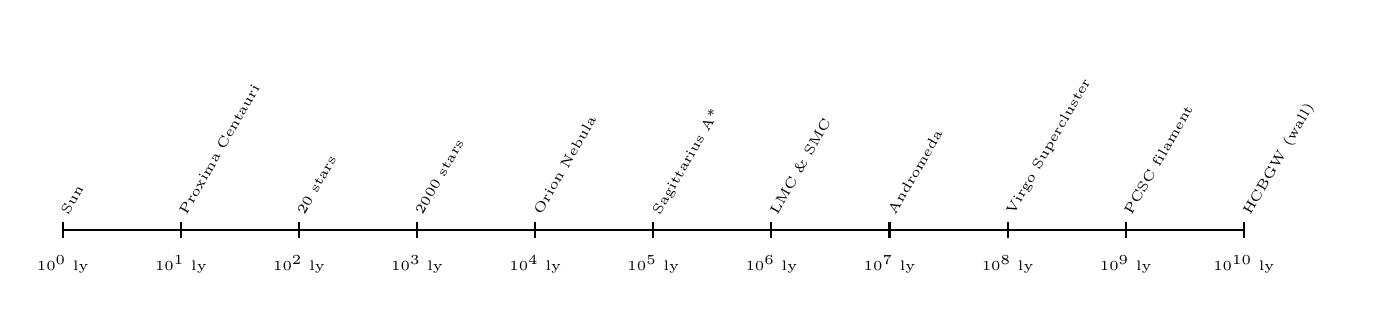
\begin{tikzpicture}
    % Parameters
    \def\n{10}
    \def\length{15}
    \def\spacing{\length/\n}

    % Labels array
    \def\labels{{"Sun", "Proxima Centauri", "20 stars", "2000 stars", "Orion Nebula", "Sagittarius A*", 
                 "LMC \& SMC", "Andromeda", "Virgo Supercluster", 
                 "PCSC filament", "HCBGW (wall)"}}

    % Draw base line
    \draw[thick] (0,0) -- (\length,0);

    % Draw tick marks, numbers and rotated labels
    \foreach \i in {0,...,10} {
        \pgfmathsetmacro{\x}{\i*\spacing}
        \draw[thick] (\x,0.1) -- (\x,-0.1); % Tick
        \node[below, font=\tiny] at (\x, -0.2) {$10^{\i}$ ly};      % Number
        
        % Multi-line labels with a 2-line approach for long labels
        \node[above, font=\tiny, text width=2.5cm, rotate=60, anchor=north west] at (\x-0.2,+0.2) 
            {\pgfmathparse{\labels[\i]}\pgfmathresult}; % Label
    }
\end{tikzpicture}
\caption{Cosmic distances span from nearby stars to the largest known structures in the universe, measured on scales of light-years, typically up to the order of 10. Each label represents either the distance to a notable astronomical object or the size of a vast cosmic region. The diameter of the observable universe is roughly 93 billion light-years, which is nearly the order of 11.}
\end{center}
\end{figure}



\subsubsection*{Milky Way in Perspective}

To develop an intuition for cosmic scales, it is instructive to compare distances across different astronomical regimes. The nearest star to the Sun, Proxima Centauri, lies at a distance of approximately 4.24 light-years. By definition, one light-year is the distance traveled by light in vacuum over one year, corresponding to about 9.46 trillion kilometers. Within a radius of 10 light-years from the Sun, roughly 20 stars are known, while nearly 2,000 stars reside within 100 light-years. More distant stellar landmarks, such as the stars forming the Orion Belt, are located at distances ranging from approximately 800 to 1,300 light-years.

The Milky Way is a barred spiral galaxy composed of several spiral arms. Its primary spiral arms include the Perseus Arm and the Scutum--Centaurus Arm, while secondary features include the Sagittarius Arm, the Norma Arm, and the Orion Spur. The Solar System is located within the Orion Spur, a minor spiral feature situated between the Perseus Arm and the Scutum--Centaurus Arm, and containing millions of stars.

\begin{figure}[htbp]
  \centering
  % Subplot 1
  \begin{subfigure}[b]{0.35\textwidth}
    \includegraphics[width=\textwidth]{../plots/0_images/Nearby_Stars.png}
  \end{subfigure}
  \hfill
  % Subplot 2
  \begin{subfigure}[b]{0.64\textwidth}
    \includegraphics[width=\textwidth]{../plots/0_images/milky_way.png}
  \end{subfigure}

  \caption{\textit{Left:} Stars located within 15ly. \textit{Right:} A segment of the Milky Way depicting the Solar System and its neighboring nebulae located in the Orion–Cygnus Arm. The Galactic Center and other minor arms - Norma and Carina–Sagittarius - are also highlighted.}
  \label{solar_system}
\end{figure}




Near the Galactic center, the Perseus and Scutum--Centaurus arms appear to originate close to the ends of the Milky Way’s central bar, known as the Long Bar, which extends roughly 15,000--16,000 light-years across the inner Galaxy. At the very center lies Sagittarius~A*, a supermassive black hole with a mass of approximately 4 million solar masses, believed to mark the dynamical nucleus of the Milky Way. Sagittarius~A* is located at a distance of about 27,000~light-years from Earth. Together, these components define the characteristic structure of the Milky Way: a flattened spiral disk with a central bulge and an extended stellar halo.


\subsubsection*{Galactic Halo and Surrounding Galaxies}

The Milky Way’s stellar disk spans approximately 100,000 light-years in diameter and is embedded within an extended, roughly spherical dark matter halo that reaches several times this scale. This halo hosts a population of satellite galaxies, stellar streams, and globular clusters. Among the most prominent satellites is the Large Magellanic Cloud (LMC), the most massive companion of the Milky Way, located at a distance of approximately 160,000 light-years ($\sim 50$ kpc). The LMC itself possesses a companion, the Small Magellanic Cloud (SMC), situated roughly 200,000 light-years ($\sim 60$ kpc) from Earth. 

To date, more than 50 satellite galaxies of the Milky Way have been identified, ranging from relatively massive systems such as the Magellanic Clouds to ultra-faint dwarf galaxies. The nearest large external galaxy is the Andromeda Galaxy (M31), located at a distance of about 2.54 million light-years ($\sim 778$ kpc). Andromeda is estimated to be two to three times more massive than the Milky Way and is expected to merge with it in several billion years.


\begin{figure}[htbp]
  \centering
  % Subplot 1
  \begin{subfigure}[b]{0.36\textwidth}
    \includegraphics[trim= 0pt 0pt 0pt 45pt, clip, width=\textwidth]{../plots/0_images/Milky_Way_side_view.png}
  \end{subfigure}
  \hfill
  % Subplot 2
  \begin{subfigure}[b]{0.63\textwidth}
    \includegraphics[width=\textwidth]{../plots/0_images/local_group.png}
  \end{subfigure}

  \caption{\textit{Left:} Side view of the Milky Way, depicting its components and satellite galaxies, notably the Large and Small Magellanic Clouds (LMC and SMC). \textit{Right:} Spatial distribution of galaxies within the Local Group, dominated by the Milky Way and Andromeda galaxies. Source: Wikipedia - Pablo Carlos Budassi (left) and Andrew Z. Colvin (right)}
  \label{milkyway}
\end{figure}



Extending the observational horizon to a radius of roughly 10 million light-years reveals a population of several dozen galaxies, dominated by the Milky Way and Andromeda as the most massive members. This ensemble, known as the Local Group, constitutes a gravitationally bound system and occupies a peripheral region of the Virgo Supercluster.

\begin{figure}[htbp]
  \centering
  % Subplot 1
    \includegraphics[width=\textwidth]{../plots/0_images/local_superclusters.png}
  \caption{Galaxy supercluster and voids within $10^9$ ly of Virgo Supercluster. Source: Andrew Z. Colvin (Wikipedia)}
  \label{voids}
\end{figure}




\subsubsection*{Galaxy Clusters and Superclusters}

At increasingly larger distances, the megaparsec (Mpc) becomes the standard unit for cosmological measurements, with $1 \mathrm{Mpc} \approx 3.26$ million light-years. The Virgo Supercluster, which includes the Local Group, the Virgo Cluster, and numerous smaller galaxy groups, extends over a scale of approximately 30--35~Mpc (corresponding to $\sim 100$ million light-years).

The Virgo Supercluster itself is a constituent of the much larger Laniakea Supercluster, a vast gravitational basin encompassing a region several hundred megaparsecs across and containing on the order of $10^{5}$ galaxies. Prominent structures within Laniakea include the Hydra--Centaurus Supercluster, the Pavo--Indus Supercluster, and the Southern Supercluster.

Near the dynamical center of Laniakea, within the Hydra--Centaurus region, lies the so-called Great Attractor---a concentration of mass inferred from galaxy peculiar velocities. Many galaxies within Laniakea, including the Milky Way, exhibit bulk motions directed toward this region under its gravitational influence.

\subsubsection*{Cosmic Web: Filaments, Walls, and Voids}

On the largest observable scales, matter in the Universe is distributed in a complex network known as the cosmic web. Superclusters such as Laniakea, Shapley, Hercules, Coma, and Perseus--Pisces are connected through extended filamentary structures composed of galaxies, gas, and dark matter. One such structure is the Pisces--Cetus Supercluster Complex, a filamentary arrangement estimated to span nearly one billion light-years in length.

Adjacent large-scale features include the Perseus--Pegasus Filament and other interconnected structures of comparable scale. Among the most extensive reported structures is the Hercules--Corona Borealis Great Wall, which may extend over several billion light-years, although its precise size and coherence remain subjects of ongoing investigation. 

Together, these filaments, sheets, and vast underdense regions known as cosmic voids form the cosmic web, which defines the large-scale architecture of the observable Universe. This hierarchical distribution of matter is illustrated schematically in Figure~\ref{scal}.

\begin{figure}[htbp]
	\includegraphics[width=\textwidth]{../plots/0_images/scales}
	\caption{Large-scale structure of the Universe illustrating the cosmic web. \textit{Source: S. Stapelberg, Structures blog from the University of Heidelberg}}\label{large_scale}
\end{figure}




\section{Historical Background and Development}

Advances in observational technology have enabled the exploration of the Universe with unprecedented depth and precision. These developments have profoundly influenced modern astronomy and cosmology, providing new insights into the origin, evolution, and large-scale structure of the cosmos. This section presents a concise overview of the historical progression of astronomical research, with particular emphasis on key discoveries and theoretical advances over the past century that have shaped contemporary cosmological thought.

\subsection{Distance Determination beyond the Galaxy: Early Twentieth Century}

Prior to the twentieth century, the Milky Way was widely believed to constitute the entirety of the Universe. The Sun was assumed to occupy a central position within this system, and the age of the Universe was thought to be far younger than current estimates. Objects now recognized as external galaxies were instead interpreted as nearby gaseous clouds within the Milky Way and were collectively referred to as \textit{spiral nebulae}. This limited understanding of cosmic scale culminated in a prolonged scientific controversy, most notably the Great Debate of 1920 between Harlow Shapley and Heber Curtis.

At the heart of this debate lay the inability to measure reliable distances to spiral nebulae. A decisive breakthrough emerged with the discovery of the period--luminosity relation for pulsating variable stars, specifically Cepheid variables, by Henrietta Swan Leavitt in 1908 and its subsequent refinement in 1912 \citep{1908leavitt,1912leavitt}. Leavitt demonstrated a tight empirical correlation between the pulsation period of Cepheids and their intrinsic luminosity, establishing that brighter Cepheids exhibit longer periods. In its modern form, this relation may be expressed as
\[
M \propto \log P,
\]
where $M$ denotes the absolute magnitude and $P$ the pulsation period.

This relation provided, for the first time, a reliable standard candle for estimating distances well beyond the confines of the Milky Way. Its application by Edwin Hubble to Cepheid variables in nearby spiral nebulae led to the unambiguous demonstration that these objects were external galaxies, thereby vastly expanding the known scale of the Universe. The role of the Leavitt Law in establishing the extragalactic distance scale is illustrated in Figure~\ref{Leavitt-Hubble}.

\begin{figure}[ht!]
	\centering
	\begin{subfigure}[t]{0.45\textwidth}
         \centering
         \includegraphics[width=0.75\textwidth]{../plots/0_images/1912_Leavitt}
	 \label{Leavitt}
     \end{subfigure}
	\hfill
     \begin{subfigure}[t]{0.49\textwidth}
         \centering
         \includegraphics[width=\textwidth]{../plots/0_images/1929_Hubble}
	     \label{Hubble}
     \end{subfigure}
	\caption{Two remarkable discoveries of early twentieth century: a) Leavitt Law: Period (in logarithmic scale) of 25 Cepheids (of Small Magellanic Cloud) correlated with their maximum and minimum brightness. \cite{1912leavitt} b) Hubble Law: Increasing recession velocity of galaxies with respect to distance suggesting an expanding Universe. \cite{1929hubble}}\label{Leavitt_Hubble}
\end{figure}



\begin{notebox}[sharp corners, width=\textwidth]{Knowledge of Distance is fundamental in astronomy.}
Distance enables us to convert the sky’s seemingly two-dimensional projection into a three-dimensional representation of the Universe. Once the distance to a bright object is known, its true luminosity can be determined, allowing us to infer its size, mass, age and other physical characteristics.
\end{notebox}



\subsection{Expansion of the Universe}

Einstein’s original cosmological model assumed a static and spatially closed Universe. To maintain such a configuration against gravitational collapse, he introduced the cosmological constant, $\Lambda$, into the field equations of general relativity \citep{1917einstein}. This modification was later rendered unnecessary by observational evidence.

In 1923, using the then state-of-the-art 100-inch (2.5~m) Hooker Telescope at Mount Wilson Observatory, Edwin Hubble observed the Andromeda \textit{spiral nebula} (M31) and resolved individual Cepheid variable stars within it. By applying the period--luminosity relation for Cepheids \citep{1925hubble}, Hubble estimated the distance to M31 to be approximately 275~kpc, placing it well beyond the confines of the Milky Way. This result effectively resolved the Shapley--Curtis Great Debate in favor of Heber Curtis, demonstrating that Andromeda is an external galaxy and establishing that the Milky Way is only one among countless galaxies in the Universe.

By extending his observations to additional galaxies, Hubble subsequently uncovered a systematic relationship between distance and radial velocity: galaxies recede from the observer with velocities proportional to their distances, expressed as
\[
v = H_0 D,
\]
where $H_0$ is the Hubble constant \citep{1929hubble}; see Figure~\ref{Leavitt-Hubble}. This empirical law provided the first direct evidence that the Universe is undergoing a global expansion, fundamentally contradicting Einstein’s earlier static model.

The Hubble constant is a cornerstone of modern cosmology, as it sets the present-day expansion rate of the Universe and provides a means to estimate its age and size. Achieving an accurate and precise determination of $H_0$ remains one of the central objectives of contemporary observational cosmology.


\subsection{The Big Bang Model: 1930s}

Independently of Hubble’s observational work, Georges Lemaître applied Einstein’s equations of general relativity to cosmology and arrived at solutions describing an expanding Universe. In 1931, he proposed that cosmic expansion originated from an extremely hot and dense initial state, an idea that later evolved into the Big Bang model \citep{1931lemaitre}.

Further theoretical developments occurred in the late 1940s, when Gamow proposed a hot early Universe model, subsequently refined by Alpher and Herman \citep{1948gamow,1948alpher}. These works predicted the existence of a relic thermal radiation field—the cosmic microwave background (CMB)—as a remnant of the early Universe, with an expected temperature of a few kelvin.

This prediction was observationally confirmed in 1965, when Arno Penzias and Robert Wilson detected an isotropic microwave signal with a temperature of $3.4 \pm 1$~K using the Holmdel Horn antenna \citep{1965penzias}. Their discovery provided compelling empirical support for the Big Bang model, which today constitutes the foundation of the standard cosmological paradigm, describing the origin, evolution, and large-scale structure of the Universe.

\subsection{Composition of Stars}

Parallel advances in quantum physics during the early twentieth century profoundly improved the understanding of stellar structure and evolution. In 1917, Arthur Eddington proposed a thermodynamic framework to explain the stability and pulsational behavior of stars, including Cepheid variables, emphasizing the role of internal pressure and energy transport \citep{1917eddington}. Building on this work, he famously hypothesized in 1920 that stellar energy is generated through the fusion of hydrogen into helium \citep{1920eddington}, a concept that was revolutionary at the time.

Further breakthroughs arose from the analysis of stellar spectra. In her 1925 doctoral dissertation, Cecilia Payne demonstrated that hydrogen and helium are by far the most abundant elements in stellar atmospheres, overturning the prevailing assumption that stellar compositions resembled that of the Earth \citep{1925payne}. Her work firmly established these elements as the dominant constituents of stars. A comprehensive theoretical description of nuclear energy generation in stars was later provided by Hans Bethe in 1939 \citep{1939bethe}, who identified the proton--proton chain and CNO cycle as the primary mechanisms of stellar nuclear fusion.

These developments represented a major turning point in astrophysics, as they established the physical basis of stellar structure and evolution. Prior to this period, the internal mechanisms governing stars---including the origin of the cyclic pulsations observed in Cepheid variables---were largely unknown.

\subsection{Age of the Universe: 1950s}

Through detailed studies of stellar populations, Walter Baade discovered that Cepheid variables comprise two distinct classes: Type~I (classical Cepheids), which are young, metal-rich, and intrinsically brighter, and Type~II (W~Virginis stars), which are older, metal-poor, and less luminous. Baade’s recalibration of the Cepheid distance scale led to a doubling of the estimated distance to the Andromeda Galaxy and a corresponding upward revision of the inferred age of the Universe from approximately 1.8 to 3.6~billion years \citep{1958baade}.

This revision was further refined by Allan Sandage, who extended the Leavitt relation to incorporate color dependence, yielding a period--luminosity--color (PLC) relation. Sandage also revised the value of the Hubble constant to approximately $75~\mathrm{km\,s^{-1}\,Mpc^{-1}}$ \citep{1958sandage}, resulting in an estimated cosmic age of order 14~billion years. This value is notably close to modern determinations of the Hubble constant and the age of the Universe.

\subsection{Technological Development: 1960s}

Despite persistent theoretical and observational challenges, technological progress has continually driven advances in astronomy. Beginning in the 1960s, the transition from photographic plates to electronic detectors marked a major transformation in observational capabilities. The introduction of charge-coupled devices (CCDs) in astronomical photometry dramatically improved sensitivity, dynamic range, and measurement precision.

The deployment of space-based observatories further revolutionized the field by enabling access to the full electromagnetic spectrum, free from atmospheric absorption and turbulence that limit ground-based observations. Together, these technological innovations laid the foundation for precision photometry and distance measurements, which are essential for the calibration of standard candles such as Cepheid variables.

\subsection{Understanding the Universe: 1990s}

A major milestone in the extragalactic distance ladder was achieved in 1998 with the incorporation of Type~Ia supernovae as standardizable candles. The development of robust empirical methods to measure distances to galaxies hosting these supernovae, calibrated using the Cepheid period--luminosity relation, extended reliable distance measurements from scales of $\sim 100$~million light-years to several billion light-years. This dramatic extension of the cosmic distance scale led to one of the most surprising discoveries in modern cosmology: the expansion of the Universe is accelerating.

This acceleration implies the presence of a component with negative effective pressure that drives the expansion of spacetime. This unknown component was termed \emph{dark energy}. Despite extensive observational and theoretical efforts, the physical nature of dark energy remains unknown. Its discovery has underscored the importance of understanding not only the geometry of spacetime but also the detailed composition of the Universe. A simplified description of the Universe can be framed in terms of its total mass--energy content and the geometry it induces, where energy appears in various forms such as mass, radiation, and thermal energy.

\begin{wrapfigure}{r}{0.45\textwidth}
	\begin{center}
		%\vspace{-1cm}
		\includegraphics[width=7cm]{../plots/0_images/uni_compo}
		\vspace{-1mm}
		\caption{The fractional composition of the Universe consists of dark energy (68 \%), dark matter (27 \%), and baryonic matter (5 \%) is depicted, with the contributions from radiation and other relativistic particles neglected.}
		\label{uni_composition}
		\vspace{-1cm}
	\end{center}
\end{wrapfigure}


In the standard cosmological framework, the Universe is composed primarily of three components: baryonic matter, dark matter, and dark energy. Ordinary, or \emph{baryonic}, matter consists of protons, neutrons, and electrons and accounts for only about $5\%$ of the total energy density of the Universe. This component forms the stars, galaxies, and large-scale structures directly observable through electromagnetic radiation.

Dark matter constitutes approximately $27\%$ of the total energy content of the Universe. It is hypothesized to possess fundamentally different properties from baryonic matter, as it neither emits nor absorbs electromagnetic radiation, rendering it invisible to direct observation. Its existence is inferred through its gravitational influence on visible matter and radiation. Strong observational evidence for dark matter arises from gravitational lensing, galaxy rotation curves, and the fine-scale anisotropies observed in the cosmic microwave background (CMB). Importantly, the interpretation of these phenomena depends critically on accurate distance measurements; for example, lensing geometries and dynamical mass estimates are highly sensitive to the assumed distances of the relevant systems. Despite its well-established gravitational effects, the physical nature of dark matter remains one of the most significant open questions in contemporary astrophysics.

Dark energy dominates the cosmic energy budget, contributing approximately $68\%$ of the total energy density of the Universe. In contrast, all other components---including radiation, neutrinos, and possible exotic particles---together contribute less than $1\%$. Determining the relative proportions of these components relies heavily on precise distance measurements across cosmic scales, as such measurements underpin estimates of luminosity, redshift, and volume, all of which are essential for reconstructing the Universe’s composition and its evolutionary history.

\subsubsection{$\Lambda$CDM Cosmological Model}

Observations of the distant Universe allow us to probe earlier cosmic epochs, as light requires finite time to traverse space. This fundamental property enables direct investigation of the Universe’s evolution. One approach to characterizing cosmic expansion involves measuring distances to the most distant observable objects, effectively constraining the size of the observable Universe and the cosmological horizon.

By combining insights from high-energy particle physics with general relativity, cosmologists have been able to model the evolution of the Universe back to fractions of a second after the Big Bang. Integrating these theoretical frameworks with a broad range of observational data has led to the formulation of the standard cosmological model, known as the $\Lambda$CDM (Lambda Cold Dark Matter) model. This model is characterized by a small set of parameters, including the densities of dark energy, dark matter, and baryonic matter; the Hubble constant ($H_0$); the scalar spectral index describing primordial density fluctuations; and the curvature parameter that determines the geometry of spacetime. Many of these parameters are tightly constrained by measurements of the cosmic microwave background and are independently supported by large-scale structure surveys, baryon acoustic oscillations, and supernova observations.

The full-sky temperature anisotropy map shown on the introductory page is a snapshot of the early Universe obtained by the \emph{Planck} satellite, a mission of the European Space Agency operational between 2009 and 2013. This map depicts the cosmic microwave background radiation, the relic thermal emission from the epoch of recombination. The small temperature fluctuations observed across the sky correspond to primordial density perturbations in the early Universe. Over billions of years, these perturbations grew through gravitational instability, ultimately giving rise to galaxies, clusters, and the large-scale structure observed today.

The CMB represents the earliest observable relic of the Universe, providing a view of conditions approximately 380{,}000~years after the Big Bang. Its precise measurement enables robust constraints on fundamental cosmological parameters, including the age, composition, and expansion rate of the Universe. Among the most significant results derived from the \emph{Planck} mission is a high-precision determination of the Hubble constant, $H_0$, which plays a central role in understanding both the past evolution and the future fate of the Universe.

\subsection{Cosmic Distance Ladder and the Hubble Constant: The Twenty-First Century}

Distance measurements across cosmic scales rely on a hierarchical set of interconnected methods collectively known as the \emph{cosmic distance ladder}, in which each rung is calibrated using more local and direct techniques. This framework allows distances to be extended progressively to cosmological scales, where they can be compared with early-Universe inferences from the cosmic microwave background (CMB).

\begin{wrapfigure}{r}{0.45\textwidth}
	\begin{center}
		\vspace{-1cm}
		\includegraphics[width=7cm]{../plots/0_images/ladder}
		\vspace{-1mm}
		\caption{An instance of Cosmic Distance Ladder calibrating Leavitt Law with parallax, SNIa with Leavitt Law and Hubble Law with SNIa based distances. \citep{2022riess}}
		\label{ladder}
		\vspace{-1cm}
	\end{center}
\end{wrapfigure}



A major refinement of the ladder was achieved by Riess and collaborators using Type~Ia supernovae (SNIa) as distance indicators. These thermonuclear explosions of white dwarfs exhibit a well-defined correlation between peak luminosity and light-curve shape, enabling their use as standardizable candles. By calibrating SNIa luminosities with Cepheid variable stars via the Leavitt Law, distances were extended from the Cepheid-accessible local volume of $\sim 30$~Mpc ($\sim 10^8$~ly) to beyond $1000$~Mpc ($\sim 10^{10}$~ly) \citep{1998riess}. 

Figure~\ref{ladder} illustrates the cosmic distance ladder, beginning with geometric parallax, progressing through Cepheids, and culminating in SNIa measurements at high redshift. Applying this calibrated framework to the Hubble--Lemaître relation yields
\[
H_0 = 73.30 \pm 1.04 \; \mathrm{km\,s^{-1}\,Mpc^{-1}},
\]
which differs by $\sim 5\sigma$ from the value inferred by \emph{Planck} CMB observations under $\Lambda$CDM assumptions \citep{2022riess,2018planck}. This persistent discrepancy, known as the \emph{Hubble tension}, may reflect unaccounted systematic uncertainties or signal new physics beyond the standard cosmological model, and remains a central challenge in contemporary cosmology.

\subsection{Golden Era of Astronomy: Gaia and Beyond (2013--Present)}

The launch of the \emph{Gaia} satellite by the European Space Agency (ESA) in 2013 marked a transformative step in precision astrophysics. By measuring geometric parallaxes with unprecedented accuracy, Gaia has determined distances to over 1.8 billion stars in the Milky Way and its surroundings, providing a definitive foundation for the calibration of standard candles such as Cepheid variable stars. These precise parallax measurements directly improve the zero-point determination of the Leavitt Law, reducing systematic uncertainties in the local distance ladder and enabling more accurate estimates of the Hubble constant ($H_0$). This work relies on distance measurements derived from Gaia Data Release 3 (DR3).

The James Webb Space Telescope (JWST), launched in 2021, complements Gaia by extending observations into the infrared, where Cepheids are less affected by dust extinction and metallicity effects. JWST’s sensitivity allows high-precision photometry of Cepheid variables in nearby and distant galaxies, further refining their period--luminosity relation and extending the reach of the cosmic distance ladder deeper into the Hubble flow.

In addition to these missions, major surveys and observatories such as SDSS, Planck, and 2dFGRS have provided critical data for cross-checking and anchoring distance measurements. Future facilities—including the Vera C. Rubin Observatory, DESI, 4MOST, Euclid, SKA, and LISA—promise to deliver even more precise observations, offering independent calibration pathways for standard candles and the local expansion rate.

Beyond photometry and astrometry, the advent of multimessenger astronomy—through the detection of cosmic rays, neutrinos, and gravitational waves—introduces alternative distance indicators, such as standard sirens, which can independently validate Cepheid- and SNIa-based distances. 

Collectively, these technological and observational advances mark the golden era of modern astronomy. By providing highly accurate distances,  they enable precise calibration of the Leavitt Law, strengthening the foundation of the cosmic distance ladder and advancing our ability to determine the Hubble constant with reduced systematic uncertainties.

\section{Scope of this Thesis}

It is evident from the previous sections that accurate distance measurements are essential in astronomy, as they underpin the determination of fundamental physical properties—such as size, mass, and age—across diverse astrophysical and cosmological contexts. Building on this principle, the primary focus of this master’s thesis is the calibration of a key distance indicator—the Leavitt Law—by minimizing systematic errors that contribute to scatter in the period--luminosity (PL) relation.


\begin{wrapfigure}{r}{0.4\textwidth}
	\begin{center}
		\vspace{-1.2cm}
		\includegraphics[width=6cm]{../plots/0_images/Storm2011.png}
		\vspace{0mm}
		\caption{\textit{K-band Period-Luminosity relation for Galactic Cepheid using IRSB distance.} Source: Storm J., 2011}\label{PLjesper}
		\vspace{-1cm}
	\end{center}
\end{wrapfigure}


Systematic uncertainties in reddening and distances of Galactic Cepheids directly affect the slope and zero-point of the PL relation, while the effect of metallicity is not considered in this thesis. Since the PL relation forms the foundation for the next rung of the cosmic distance ladder, even small errors can propagate and amplify at larger scales. Achieving a precise and well-constrained PL relation is therefore crucial for reliable cosmological measurements. In this thesis, the refinement of the Leavitt Law is implemented through a structured methodology, summarized as follows:

\begin{itemize}
    \item Identify and remove outliers from the BVIJHK photometric dataset of Galactic Cepheids.
    \item Refine the Galactic reddening law \cite{2007fouque} to minimize deviations between apparent and absolute magnitudes using Wesenheit functions.
    \item Estimate absolute luminosities of Cepheids using band-wise extinction corrections and distances derived from the Infrared Surface Brightness (IRSB) method \cite{2011jesper} and Gaia parallaxes \cite{2023gaia}.
    \item Develop and adapt a mathematical framework for PL calibration based on \cite{2017madore} to improve error corrections.
    \item Quantify uncertainties in distances and interstellar reddenings for individual Cepheids following the refined methodology.
    \item Derive the calibrated Leavitt Law using distance- and reddening-corrected absolute magnitudes.
    \item Cross-validate the calibrated PL relation with Cluster Cepheids \cite{2023cruz}.
    \item Apply the refined Leavitt Law to Cepheids in the Large and Small Magellanic Clouds to determine their distances.
\end{itemize}

This thesis is organized into three parts. The first part presents the physics of Cepheid pulsation. The second part develops the calibration methodology for addressing distance and reddening systematics. The final part presents the calibrated Leavitt Law, discusses its implications for the extragalactic distance scale through applications to the Magellanic Clouds, and concludes with prospects for future work.

\subsection{Part I: Parameters of the Leavitt Law}
The period--luminosity (PL) relation depends on two key parameters of Cepheid variables: (a) the pulsation period and (b) the intrinsic (absolute) luminosity. Figure~\ref{PLjesper} illustrates the Leavitt Law in the $K$ band, with distances measured via the Infrared Surface Brightness (IRSB) method \citep{2011storm} and interstellar extinction estimated using Fouqué's law \citep{2007fouque} combined with Fernie's reddening measurements \citep{1994fernie}.

Pulsation periods are derived from light curves spanning multiple cycles and are well-determined for all targets in this study. The focus of this thesis is on accurately estimating intrinsic luminosities, which requires correcting the observed apparent magnitudes for both distance and interstellar extinction.

Stellar light is attenuated by scattering and absorption in the interstellar medium, particularly by dust and gas along the line of sight. Inaccurate corrections can introduce significant deviations from the expected linear PL relation. Therefore, a central objective of this thesis is to quantify uncertainties in both distance and reddening for each Cepheid and assess their impact on the PL relation.

This first part of the thesis is devoted to examining these parameters, their interdependencies, and the methodologies employed for their determination.

\subsection{Part II: Calibration Method and Dataset}

This part of the thesis covers the Galactic Cepheid dataset, the calibration methodology, the underlying physics, and comparison analyses. The dataset includes multiband photometry in the BVIJHK bands. Color excesses compiled by Fernie \citep{1994fernie} are converted to band-specific extinction using the Cardelli et al. law \citep{1989cardelli} combined with the total-to-selective extinction ratio from Sandage \citep{2004sandage}. Leavitt Laws are then derived using both Gaia parallaxes and IRSB distances, corrected for extinction. Prior to calibration, deviations in the slope and intercept of the Leavitt Law for both distance estimates are examined.

The calibration follows Madore's approach \citep{2017madore}, which employs the reddening-free Wesenheit function \citep{1982madore} to decouple reddening and distance errors. Unlike Madore, who applied a single Wesenheit relation for all residual correlations, this thesis compares residuals from the BVIJHK period--luminosity relations with corresponding composite period--Wesenheit relations. While Madore used only the $V-I$ Wesenheit function, this study extends the method to all fifteen color indices derived from BVIJHK photometry to compute distance--reddening error pairs for each star. Further extending the method to composite Wesenheit functions reveals how period–Wesenheit residuals depend on reddening ratios and color indices.

Finally, the calibrated Leavitt Law is cross-validated using 18 Galactic cluster Cepheids \cite{cruz2023}, whose distances are more reliably determined from the averaged parallaxes of their host clusters. This part concludes with an analysis of the calibration results and their implications for refining the PL relation.

\subsection{Part III: Results and Prospects for Improvement}

\subsubsection*{LMC and SMC Distances}
To evaluate the effectiveness of the calibration, distances to the Large and Small Magellanic Clouds (LMC and SMC) are derived using 24 versions of the calibrated Leavitt Law, covering four photometric bands (VIJK) and six color-based Wesenheit functions. This approach allows the construction of a distance matrix that highlights the relative performance of different color indices in producing consistent distance estimates. The results demonstrate the sensitivity of the PL calibration to the choice of photometric band and Wesenheit function, providing guidance for selecting the most robust combination for extragalactic distance determinations.

\subsubsection*{Effect of Metallicity}
While metallicity can affect the zero-point and slope of the period--luminosity relation, it is not explicitly considered in this thesis. However, the framework developed here is readily extendable to incorporate metallicity corrections in future studies, enabling a more comprehensive calibration of the Leavitt Law across different galactic environments.

\subsubsection*{Target-Based Reddening Law}
The refined calibration methodology also provides insights into the reddening law for individual Cepheids. By comparing observed deviations across multiple bands and Wesenheit functions, star-specific reddening ratios can be inferred, allowing a more precise correction of extinction effects. This target-based approach can improve the accuracy of distance estimates, particularly in regions with non-standard or spatially varying extinction, and serves as a foundation for further refinement of both Galactic and extragalactic distance measurements.

\subsubsection*{Prospects for Further Improvement}
The methodology presented here can be extended in several ways: 
\begin{itemize}
    \item Incorporating metallicity corrections to account for chemical composition effects on the PL relation.
    \item Expanding the dataset to include additional Galactic and extragalactic Cepheids for improved statistical robustness.
    \item Integrating multi-wavelength data from upcoming surveys (e.g., JWST, LSST) to refine extinction corrections and Wesenheit function formulations.
\end{itemize}
Together, these improvements will enhance the precision and reliability of the Leavitt Law, thereby reducing systematic uncertainties in the cosmic distance ladder and advancing our understanding of the scale and expansion of the Universe.
